\documentclass[../main.tex]{subfiles}

\begin{document}
\قسمت{درباره جنگ ستارگان}

\زیرقسمت{مقدمه}
همانطور که در طول درس هم متوجه شده‌اید، پرهام مجموعه فیلم‌های جنگ ستارگان\پانویس{The Star Wars} را دوست دارد.
در این آزمون قصد داریم یک وب‌سایت ساده برای جمع‌آوری اطلاعات این مجموعه فیلم طراحی کنیم.

\زیرقسمت{وب‌گاه}
\paragraph{}
وب‌گاهی که پیاده‌سازی می‌کنید، از شمای زیر پیروی می‌کند. در این شِما یک عکس پس‌زمینه وجود داشته و محتوا در قالب یک مستطیل با پس‌زمینه شفاف روی آن نمایش داده می‌شود.
در نظر داشته باشید که عکس پس‌زمینه می‌بایست تمام صفحه را پوشانده باشد و در صورتی که از صفحه بزرگتر باشد \متن‌سیاه{نباید} باعث ایجاد \متن‌لاتین{scrollbar} گردد.
در شرایطی که ابعاد صفحه نمایش مناسب نباشد می‌بایست قسمتی از وسط عکس نمایش داده شود.
برای تصویر پس‌زمینه حتما از عکس استفاده کنید، برای مثال می‌توانید از \تارنما{https://unsplash.com/s/photos/starwars}{اینجا} استفاده کنید.

\شروع{شکل}[h]
  \تنظیم‌ازوسط
  \درج‌تصویر[scale=0.25]{./swapi-top-level}
  \شرح{طراحی سطح بالا}
\پایان{شکل}

مستطیل میانی تمامی محتویات قابل نمایش شما را می‌بایست شامل شود. این مستطیل می‌بایست تنها به اندازه محتویات باشد اما برای نمایش زیباتر برای آن \متن‌لاتین{padding} در نظر بگیرید.
محتوای مورد نمایش شما، ۱۰ مورد اول از کشتی‌فضایی\پانویس{Starship}های مجموعه جنگ‌ستارگان برگرفته از تارنمای زیر می‌باشد:

\begin{latin}
  \url{https://swapi.dev/}
\end{latin}

توجه داشته باشید که در اینجا لزوما تمام شناسه‌ها موجود نمی‌باشند بنابراین ۱۰ کشتی‌فضایی اول لزوما شناسه‌ی ۱ تا ۱۰ نخواهند داشت.

\شروع{امتیازی}
پیاده‌سازی صفحه‌گذاری\LTRfootnote{pagination}.
\پایان{امتیازی}

\شروع{امتیازی}
هندل کردن صحیح خطاهای \متن‌لاتین{API} با نمایش پیام خطا
\پایان{امتیازی}

\begin{figure}[h]
  \centering
  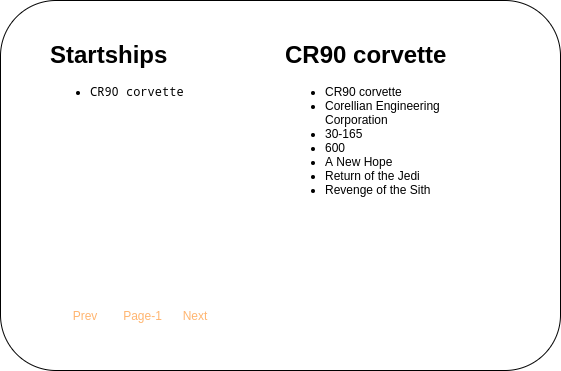
\includegraphics[scale=0.25]{./swapi-content}
  \caption{طراحی مستطیل محتوا}
\end{figure}

\paragraph{}
کاربر می‌تواند از لیست این کشتی‌فضایی‌ها یکی را انتخاب کرده و جزئیات آن را ببیند.
اگر بخواهیم دقیقتر صحبت کنیم لیست شامل \متن‌ایتالیک{نام} ۱۰ کشتی‌فضایی است
که با کلیک بر روی هر یک اطلاعات جزئی آن شامل \متن‌اتالیک{مدل}، \متن‌ایتالیک{سازنده}، \متن‌ایتالیک{خدمه} و \متن‌ایتالیک{تعداد مسافران} نمایان می‌گردد.
برای نمونه داده‌ای که شما برای یک کشتی فضایی دریافت می‌کنید در ادامه آورده شده است.

\begin{latin}
\begin{minted}[bgcolor=LightGray]{json}
{
    "name": "Imperial shuttle",
    "model": "Lambda-class T-4a shuttle",
    "manufacturer": "Sienar Fleet Systems",
    "cost_in_credits": "240000",
    "length": "20",
    "max_atmosphering_speed": "850",
    "crew": "6",
    "passengers": "20",
    "cargo_capacity": "80000",
    "consumables": "2 months",
    "hyperdrive_rating": "1.0",
    "MGLT": "50",
    "starship_class": "Armed government transport",
    "pilots": [
        "http://swapi.dev/api/people/1/",
        "http://swapi.dev/api/people/13/",
        "http://swapi.dev/api/people/14/"
    ],
    "films": [
        "http://swapi.dev/api/films/2/",
        "http://swapi.dev/api/films/3/"
    ],
    "created": "2014-12-15T13:04:47.235000Z",
    "edited": "2014-12-20T21:23:49.900000Z",
    "url": "http://swapi.dev/api/starships/22/"
}
\end{minted}
\end{latin}

در صورتی که قسمت فیلم‌ها نیز دارای اطلاعات باشد می‌بایست نام فیلم‌ها ذکر شود.
دقت کنید برای این امر نیاز به یک تقاضای جداگانه برای فیلم دارید. ساختار \متن‌لاتین{URL}ها در اینجا بسیار ساده می‌باشند ولی در جهت تاکید در قسمت زیر آن‌ها را مرور کرده‌ایم:

\begin{itemize}\begin{latinitems}
  \item https://swapi.dev/api/starships/<id>
  \item https://swapi.dev/api/films/<id>
\end{latinitems}\end{itemize}

\زیرقسمت{صفحه‌گذاری}

فرض کنید لیست بلندی از آیتم‌ها در اختیار شما قرار گرفته است، در صفحه‌گذاری این لیست را به صفحاتی می‌شکانید که در هر صفحه تعداد مشخصی از اطلاعات وجود دارند. کاربران به جای کارکردن با لیست بلندی از آیتم‌ها با صفحاتی مواجه هستند که تعداد مشخصی از آیتم‌ها را در بر گرفته‌اند. کاربر می‌تواند از قبل در رابطه با تعداد کل صفحات اطلاع داشته باشد و می‌تواند چنین اطلاعی نیز به او داده نشود. همانطور که ادامه هم بیان می‌شود چگونگی پیاده‌سازی این موضوع به خود شما وابسته است.
جزئیات پیاده‌سازی این قسمت کاملا برعهده خودتان می‌باشد.
می‌توانید لیست تمام کشتی‌فضایی‌ها را در ابتدا ساخته و در ادامه صفحه‌گذاری را کاملا در سمت کلاینت انجام دهید یا می‌توانید در هر بار تغییر صفحه لیست کشتی‌فضایی‌ها را دریافت کنید.
در نظر داشته باشید که تمامی فرآیند می‌بایست پویا بوده باشد و هیچ چیز به صورتی دستی در کدتان وارد نشده باشد، به طور دقیق‌تر با تغییر تعداد کشتی‌فضایی‌ها می‌بایست همچنان برنامه شما به طور صحیح به فعالیت خود ادامه دهد.

به طور مثال فرض کنید در مجموع ۲۶ کشتی‌فضایی وجود دارند. یک راه برای پیاده‌سازی صفحه‌گذاری به این ترتیب خواهد بود.

\شروع{شمارش}
  \فقره گرفتن تمامی اطلاعات کشتی‌فضایی‌های موجود
  \فقره نمایش ۱۰ کشتی‌فضایی در هر صفحه، به این ترتیب دو صفحه با ۱۰ کشتی‌فضایی و یک صفحه با ۶ کشتی‌فضایی خواهیم داشت.
  \فقره پیاده‌سازی دکمه‌هایی برای جابجایی بین صفحات
\پایان{شمارش}

\زیرقسمت{نکات پیاده‌سازی}

\شروع{فقرات}
\فقره آنچه در شما آورده شده است برای فهم بهتر شما می‌باشد بنابراین سعی کنید تا حد امکان وب‌سایت را گویا طراحی کنید.
\فقره برای کدهایتان از کامنت استفاده کنید. توضیح کارکرد بلاک‌های \متن‌لاتین{css} اجباری می‌باشد. توابعی و قطعات کد جاوا اسکریپت نیز می‌بایست حداقل یک خط کامنت داشته باشند.
\فقره کامنت فارسی یا انگلیسی موردی ندارد اما از فینگلیش (!) نوشتن پرهیز کنید.
\فقره استفاده از کتابخانه‌ها و فریم‌ورک‌ها در پروژه مجاز \متن‌سیاه{نمی‌باشد}.
\فقره از آنجایی که این پروژه در قالب \متن‌سیاه{امتحان میانترم} می‌باشد از تغییر دادن صورت مساله یا انجام موارد خارج از موارد مطرح شده خودداری کنید.
\پایان{فقرات}

\subsection{پرسش‌های متداول}

\begin{enumerate}
  \item منظورتان از این که "درصورتی که ابعاد صفحه مناسب نباشد عکس در وسط زوم شود" چیست؟ مگه قرار نیست عکس ما کل صفحه رو بپوشاند و متناسب با تغییرات صفحه اندازه‌اش نیز تغییر کند؟\\
        ببینید عکسی که انتخاب می‌کنید قاعدتا یک اندازه مشخصی دارد که اگر در صفحه جا نشود به اجبار می‌بایست قسمتی از آن را نمایش دهید، منظور من این بود که این قسمت از وسط عکس بریده شده باشد.
  \item برای اطلاعاتی که داخل مستطیل میانی قابل نمایش است، ابتدا باید همه سفینه‌ها در سمت چپ صفحه مشخص باشند، سمت راست اطلاعات هر سفینه انتخابی باشد؟ یا فرمتی که این ها میتونن قرار بگیرند خیلی مهم نیست؟\\
        فرمت کلی به این شکل است اما هر تغییری در این قسمت ممکن است.
  \item هندل کردن \lr{404 Not Found}‌های \lr{api} چطوری باید باشد؟\\
        در حالت اجباری تنها لیست کردن ۱۰ کشتی‌فضایی لازم است. شما برای این امر حتی می‌توانید \textbf{شناسه‌های} ۱۰ کشتی‌فضایی را به صورت دستی بدست آورده و در کد لیست کنید.
  \item کدهای \lr{js} و \lr{html} در چه حد کامنت لازم دارند؟ اگر اسم متغیرها و متدها گویا باشند باز هم لازم است؟\\
        در رابطه با \lr{html} تنها نیاز است که قسمت‌های کلی را معرفی کنید، به طور مثال مشخص کنید از این بخش برای لیست کردن کشتی‌فضایی‌ها استفاده خواهید کرد. در رابطه \lr{js} در صورتی که از نام‌های مناسب برای توابع و متغیرهای استفاده کنید کفایت خواهد کرد. در رابطه با \lr{css} همانطور که بیان شد توضیح بلاک‌ها اجباری می‌باشد. به طور مثال این بلاک قصد دارد عکس پس زمینه با که با \lr{\#background} مشخص شده است را در تمام صحفه نمایش داده و در وسط قرار دهد.
\end{enumerate}

\end{document}
